\documentclass{article}

%%%%%%%%%%%%%
\oddsidemargin 0.0in
\evensidemargin 0.0in
\textwidth 6.0in
%\headheight 1.0in
%\topmargin 0.5in
%\textheight 9.0in
%\footheight 1.0in
%%%%%%%%%%%% 

\usepackage{graphicx}

\title{Tricubic Engine\\
Technical Notes and Full Matrix}

\author{Francois Lekien, Chad Coulliette and Jerry Marsden\\
California Institute of Technology}

\begin{document}

\maketitle

\begin{abstract}
The objective of this paper is to document a local interpolation scheme in three dimensions, available as a package called \verb+tricubic+. In contrast to global interpolation where the interpolated function usually depends on the whole data set, local interpolation only uses data in a neighborhood of an element. 
The function interpolated with the tricubic interpolator and its three first derivatives are continuous. As shown in Lekien, Coulliette and Marsden, 2004, this is the only cubic $C^1$ local interpolator.
The implementation of the interpolator can be downloaded as a static and dynamic library for most platforms.
\end{abstract}

\tableofcontents

\section{Interpolator Equation}

We assume that the value of the function $f$ is given at the corners of a regular mesh (see Fig.~\ref{figcube}). The function $f$ to interpolate is represented in each element by

\begin{figure}
\centering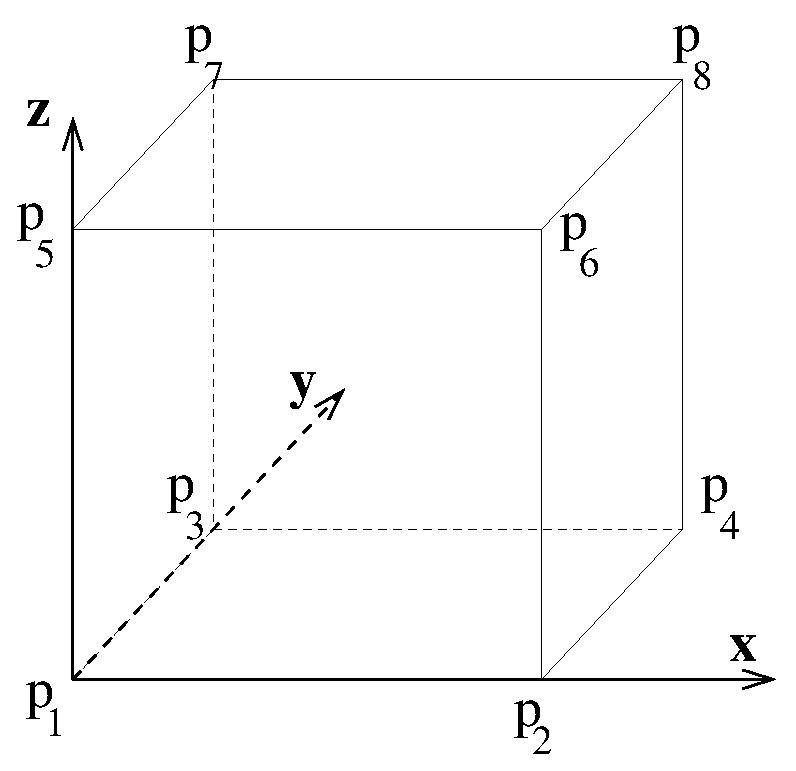
\includegraphics[width=3in]{1cube}
\caption{Element for interpolation in three dimensions.}
\label{figcube}
\end{figure}

\begin{equation}
f(x,y,z) = \sum _{i=0}^{N} \sum _{j=0}^{N} \sum _{k=0}^{N} a_{i j k} x^i y^j z^k \; .
\label{fpoly3}
\end{equation} The coefficients $a_{i j k}$ are determined in Lekien, Coulliette and Marsden,~2004  in such a way that the function $f$ described by Eq.~\ref{fpoly3} is $C^1$, i.e. $f$ is continous and its 3 first derivatives are also continuous.

For the sake of simplicity, the 64 coefficients $a_{i j k}$ are stacked in a vector $\bar{\alpha }$ by defining
\begin{equation}
\alpha _{1+i+4 j+16 k} = a_{i j k} \; \; \; \forall i,j,k \in \left\{ 0 , 1 ,2 ,3 \right\} \; .
\end{equation}

\noindent Similarly, we give a unique indice to each corner of the cube as shown in Fig.~\ref{figcube}. We stack the constraints on $f$ and its derivatives in a vector $\bar{b}$ by defining
\begin{equation}
b_i = \left\{
\begin{array}{lcl}
f(p_i)&if&1\leq i \leq 8\\
\frac{\partial f}{\partial x}(p_{i-8})&if&9\leq i \leq 16\\
\frac{\partial f}{\partial y}(p_{i-16})&if&17\leq i \leq 24\\
\frac{\partial f}{\partial z}(p_{i-24})&if&25\leq i \leq 32\\
\frac{\partial ^2 f}{\partial x \partial y}(p_{i-32})&if&33\leq i \leq 40\\
\frac{\partial ^2 f}{\partial x \partial z}(p_{i-40})&if&41\leq i \leq 48\\
\frac{\partial ^2 f}{\partial y \partial z}(p_{i-48})&if&49\leq i \leq 56\\
\frac{\partial ^3 f}{\partial x \partial y \partial z}(p_{i-56})&if&57\leq i \leq 64\\
\end{array}
\right.
\end{equation}

\noindent Based on Eq.~\ref{fpoly3}, the derivatives of $f$ can be computed and evaluated for the $8$ points $p_i$. This gives a linear system in the 64 unknown coefficients $\alpha _i$
\begin{equation}
B \bar{\alpha } = \bar{b} \; ,
\end{equation} The matrix $B$ is $64\times 64 $ and has only integer entries. It can be computed by a computer program. The elements of the matrix $B$ are irrelevant for the methods, so we do not give them in this document. It is important to note that the determinant of $B$ is
\begin{equation}
\det \left( B \right) = 1 \; .
\end{equation}

\noindent As a result, $B$ is invertible and the coefficient $\alpha _i$ can be computed using the linear relationship
\begin{equation}
\bar{\alpha } = B^{-1} \bar{b} \; . 
\label{Binv}
\end{equation} The matrix $B^{-1}$ is the core of the tricubic interpolator. It can be found in Table~\ref{Binv1} to Table~\ref{Binv8}.


\begin{table}
\begin{center}
\input{Binv1}
\end{center}
\caption{Part1}
\label{Binv1}
\end{table}

\begin{table}
\begin{center}
\input{Binv2}
\end{center}
\caption{Part2}
\label{Binv2}
\end{table}

\begin{table}
\begin{center}
\input{Binv3}
\end{center}
\caption{Part3}
\label{Binv3}
\end{table}

\begin{table}
\begin{center}
\input{Binv4}
\end{center}
\caption{Part4}
\label{Binv4}
\end{table}

\begin{table}
\begin{center}
\input{Binv5}
\end{center}
\caption{Part5}
\label{Binv5}
\end{table}

\begin{table}
\begin{center}
\input{Binv6}
\end{center}
\caption{Part6}
\label{Binv6}
\end{table}

\begin{table}
\begin{center}
\input{Binv7}
\end{center}
\caption{Part7}
\label{Binv7}
\end{table}

\begin{table}
\begin{center}
\input{Binv8}
\end{center}
\caption{Part8}
\label{Binv8}
\end{table}

\section{Numerical Implementation}

An algorithm using the tricubic interpolator consist of the following 3 steps:
\begin{itemize}
\item Vector $\bar{b}$. The values of $f$ and the derivatives at the 8 corners of the cube must be stacked in vector of dimension $64$. The values of $f$ are usually given at the corner and the derivatives can be evaluated by finite differences and the boundary conditions. Notice that the method described here assumes a cube of side $1$. As a result, of the cube has arbitrary sides $\delta _x$,$\delta _y$, and $\delta _z$, the derivatives in $x$, $y$, $z$ must be respectively multiplied by $\delta _x$, $\delta _y$ and $\delta _z$. For example, if the derivative $\partial ^2 \partial x \partial y$ is computed in the initial cube, it must be multiplied by $\delta _x . \delta y$ before computing the tricubic coefficients.
\item Vector $\bar{\alpha }$. The value of the coefficients are computed using the relation $\bar{\alpha } = B^{-1} \bar{b}$.
\item Value of the function. The value of the function $f$ can be computed at any point of the cube by the relationship given by Eq.~\ref{fpoly3}. Notice that the coordinates $x$, $y$, $z$ are relative to the unit cube. In other words, the coordinates $x$, $y$, and $z$ must be translated to the corner $p_1$ of the cube and scaled respectively by $\delta _x$, $\delta _y$ and $\delta _z$. If the value of the derivatives of the function $f$ are needed, one can differentiate Eq.~\ref{fpoly3} with respect to any set of variables and get a form for the derivatives of $f$. Notice that the derivatives are given in terms of the unit cube and must be divided by the actual size of the elements. In other words, the value of $\partial ^{i+j+k} f / \partial x^i \partial y^j \partial z^k$ must be divided by $\delta _x^i \delta _y^j \delta _z^k$.
\end{itemize}

\noindent This algorithm has been implemented in a library called \verb+libtricubic+ and is available for download at {\em http://gyre.cds.caltech.edu/software/tricubic }. Programs using the tricubic library usually have an include line that imports the prototype of the tricubic function
\begin{verbatim}
#include ``tricubic.h''
\end{verbatim}
The source code is usally linked with the tricubic library with the following arguments
\begin{verbatim}
gcc source.cpp -L/path/to/tricubiclib/ -ltricubic
\end{verbatim}

\noindent If the installation of libtricubic is system-wide (i.e. run \verb+make install+ as \verb+root+), the above code and command are simplified to
\begin{verbatim}
#include <tricubic.h>
\end{verbatim}
The source code is usally linked with the tricubic library with the following arguments
\begin{verbatim}
gcc source.cpp -ltricubic
\end{verbatim}

\noindent The functions available in the library are
\begin{itemize}
\item \verb+char *tricubic_version(void)+. Returns a string containing the version of the library.
\item \verb+void tricubic_get_coeff(double a[64], double f[8], double dfdx[8], double dfdy[8],+\\\verb+   double dfdz[8],double d2fdxdy[8], double d2fdxdz[8], double d2fdydz[8],+\\\verb+   double d3fdxdydz[8])+. Takes 8 vectors of dimension $8$ containing the value of $f$ and the required derivatives for each point of Fig.~\ref{figcube}. Returns the $64$ coefficients of the tricubic interpolation in \verb+a[64]+.
\item \verb+double tricubic_eval(double a[64], double x, double y, double z,+\\\verb+                     int derx, int dery, int derz)+. Takes the 64 coefficients \verb+a[64]+ as input and compute a value at point \verb+x+,\verb+y+,\verb+z+. The three coordinates are given with respect to the corner $p_1$ in Fig.~\ref{figcube} and are scaled in such a way that the element is a cube of side 1. The function computed is \begin{equation}
\frac{\partial ^{derx+dery+derz} f}{\partial x^{derx} \partial y^{dery} \partial z^{derz}} \; ,
\end{equation} where we use the convention $f = \frac{\partial ^0}{\partial x^0 \partial y^0  \partial z^0 }$ to compute the value of the function $f$.
\item \verb+double tricubic_eval(double a[64], double x, double y, double z)+. Shortcut for the previous function with \verb+derx+$=$\verb+dery+$=$\verb+derz+$=0$.
\end{itemize}

\section{Example}

\begin{verbatim}
/************************************************************/
/* example1.cpp : illustrates the use of libtricubic        */
/* Francois Lekien <lekien@mit.edu> 2004-01-20              */
/************************************************************/

///Required Include File: tricubic.h
///If tricubic.h has not been installed in a directory
///  accessible by the compiler, use -I/path/to/tricubic
#include <tricubic.h>

///Define the box
///Tricubic is written for cubes of side 1. Multiplications and
///  divisions are needed along the way for rectangular box with
///  arbitrary sides. See below for details.
#define dx 0.2
#define dy 2.0
#define dz 0.3

///These are the 8 functions that need to be known at the 8 corners.
///The functions are f, the three first derivatives dfdx, dfdy, dfdz,
///  the 3 mixed 2nd order derivatives and the mixed 3rd order derivative.
///The derivatives can be obtained by numercal differentiation of f at the
///  other corners of the grid. See Numerical Recipies for examples in 2D
///The order of the points is as follow:
///  0: x=0; y=0; z=0;
///  1: x=1; y=0; z=0;
///  2: x=0; y=1; z=0;
///  3: x=1; y=1; z=0;
///  4: x=0; y=0; z=1;
///  5: x=1; y=0; z=1;
///  6: x=0; y=1; z=1;
///  7: x=1; y=1; z=1;
///For convenience, the ordering of the points is available at run time
///   using tricubic_pointID2xyz(). See man page for details
double fval[8]={1.2, 2.3, 3.4, 4.5, 5.6, 6.7, 7.8, 8.9};
double dfdxval[8]={1.2, 2.3, 3.4, 4.5, 5.6, 6.7, 7.8, 8.9};
double dfdyval[8]={1.2, 2.3, 3.4, 4.5, 5.6, 6.7, 7.8, 8.9};
double dfdzval[8]={1.2, 2.3, 3.4, 4.5, 5.6, 6.7, 7.8, 8.9};
double d2fdxdyval[8]={1.2, 2.3, 3.4, 4.5, 5.6, 6.7, 7.8, 8.9};
double d2fdxdzval[8]={1.2, 2.3, 3.4, 4.5, 5.6, 6.7, 7.8, 8.9};
double d2fdydzval[8]={1.2, 2.3, 3.4, 4.5, 5.6, 6.7, 7.8, 8.9};
double d3fdxdydzval[8]={1.2, 2.3, 3.4, 4.5, 5.6, 6.7, 7.8, 8.9};

int main(int narg, char *arg[]) {
  double a[64];
  double f1, f2, dfdx, d2fdxdy;
  int i;
  double x,y,z;
  ///First we compute the 64 coefficients for the cube.
  ///The first step is to scale the derivatives that have been computed
  ///  in a rectangular box instead of the cube of side 1.
  ///Notice that this step can be avoided by computing the numerical
  ///  derivatives without dividing by the length of the boxes.
  for (i=0;i<8;i++) {
    fval[i]*=1.0;
    dfdxval[i]*=dx;
    dfdyval[i]*=dy;
    dfdzval[i]*=dz;
    d2fdxdyval[i]*=dx*dy;
    d2fdxdzval[i]*=dx*dz;
    d2fdydzval[i]*=dy*dz;
    d3fdxdydzval[i]*=dx*dy*dz;
  } 
  ///Next we get the set of coefficient for this cube
  tricubic_get_coeff(a,fval,dfdxval,dfdyval,dfdzval,d2fdxdyval,
                                d2fdxdzval,d2fdydzval,d3fdxdydzval);
  ///To get the value in the middle of the cube, we always use (.5,.5,.5)
  ///  i.e. relative coordinates
  f1=tricubic_eval(a,.5,.5,.5);
  ///To get the value at a point x,y,z (with referrence to corner ID 0
  ///  we devide by each length
  f2=tricubic_eval(a,x/dx,y/dy,z/dz);
  ///Derivatives can be computed similarly but need to be scaled by dx,dy,dz
  dfdx=tricubic_eval(a,x/dx,y/dy,z/dz,1,0,0)/dx;
  d2fdxdy=tricubic_eval(a,x/dx,y/dy,z/dz,1,1,0)/(dx*dy);
}

\end{verbatim}

\section{Further reading, Comments, Remarks and Bugs}

The proofs of $C^1$ continuity and the uniqueness of the tricubic $C^1$ interpolator has been published in the {\em International Journal for Numerical Methods in Mechanical Engineering}. See {\em F.~Lekien, C.~Coulliette and~J.~Marsden, Tricubic Interpolation, IJNME vol ??, pp 1--10, 2004} for more details.
Send comments, remarks and bug reports to Francois Lekien, Caltech 107-81, 1201 East California blvd, Pasadena, CA 91125 or lekien@mit.edu.

\end{document}
